\documentclass[12pt,a4paper]{article}
\usepackage{fullpage}
\usepackage[top=2cm, bottom=4.5cm, left=2.5cm, right=2.5cm]{geometry}
\usepackage{amsmath,amsthm,amsfonts,amssymb,amscd}
\usepackage{lastpage}
\usepackage{enumerate}
\usepackage{fancyhdr}
\usepackage{mathrsfs}
\usepackage{xcolor}
\usepackage{graphicx}
\usepackage{listings}
\usepackage{hyperref}
\usepackage{txfonts}
\usepackage{titlesec}

\hypersetup{%
  colorlinks=true,
  linkcolor=blue,
  linkbordercolor={0 0 1}
}


\newcommand\course{8.03x - Vibrations and Waves}
\newcommand\hwnumber{1}               
\newcommand\MyName{Syed Suhaib Ahmad}
 
\renewcommand\lstlistingname{Algorithm}
\renewcommand\lstlistlistingname{Algorithms}
\def\lstlistingautorefname{Alg.}

\setlength{\parindent}{0.0in}
\setlength{\parskip}{0.05in}



\pagestyle{fancyplain}
\headheight 35pt
\lhead{\course}
\chead{\large\textbf{Problem Set 1}}
\rhead{\MyName{}}
\lfoot{}
\cfoot{\small\thepage}
\rfoot{}
\headsep 1.5em

\begin{document}

\subsubsection*{Problem 1.1 - Manipulation of complex vectors}
\begin{enumerate}
    \item[(a)]Find the magnitude and direction of the vector $\left(4-\sqrt{5}j\right)^3$. 
    \item[(b)]What is the real and imaginary part of
    \[\frac{Ae^{j(\omega t+\pi/2)}}{4+5j}\]
    assuming that $A$ and $\omega$ are real?
    \item[(c)]Write the following complex vectors $Z$ in terms of $a+jb$ ($a$ and $b$ are real). Notice there may be more than one solution. 
    \[Z_1=(j)^j\,\,\,\,\,\,\,\,\,\,\,\,\,\,\,\,\,\,\,\,\,\,\,\,\,\,\,\,\,\,\,Z_2=(j)^{8.03}\]
\end{enumerate}
\textbf{Solution(a)}
\\
\\The vector is of the form $(z)^3$ and can be written as a complex exponential using Euler's formula, but first we find the magnitude and argument of $z$.
\[\text{Arg}\,z=\tan^{-1}\left(\frac{-\sqrt{5}}{4}\right)=-0.5097,\,\,\,\,\,|\,z\,|=\sqrt{(-\sqrt{5})^2+(4)^2}=\sqrt{21}.\]
Thus,
\[(z)^3=\left(\sqrt{21}e^{j(-0.5097)}\right)^3.\]
This means the direction of $z$ is scaled up by a factor of three and magnitude is raised to the power of three.
\[\text{Direction of }(z)^3=3\tan^{-1}\left(\frac{-\sqrt{5}}{4}\right)=-1.529\,\text{rad}=-87.6\text{°},\]
\[\text{Magnitude of }(z)^3=\left(\sqrt{21}\right)^3=96.2.\]
\textbf{Solution(b)}
\\
\\Let the given expression is $\zeta=\frac{Ae^{j(\omega t+\pi/2)}}{z}$ where $z=4+5j$ and can be expressed a complex exponential in the following way
\[z=\sqrt{5^2+4^2}e^{j\tan^{-1}\left(\frac{5}{4}\right)}=\sqrt{41}e^{j\theta}\,\,\,\,\,\,\,\,\,\,\text{where}\,\,\,\,\,\,\,\,\,\,\theta=\tan^{-1}\left(\frac{5}{4}\right).\]
Now we have a simplified form of $\zeta$.
\[\zeta=\frac{Ae^{j(\omega t+\pi/2)}}{\sqrt{41}e^{j\theta}}=\frac{A}{\sqrt{41}}e^{j(\omega t+\pi/2-\theta)}=\frac{A}{\sqrt{41}}(\cos(\omega t+\pi/2-\theta)+j\sin(\omega t+\pi/2-\theta)).\]
Finally,
\[\text{Re }\zeta=\frac{A}{\sqrt{41}}\cos(\omega t+\pi/2-\theta)\,\,\,\,\,\,\,\,\,\,\text{and}\,\,\,\,\,\,\,\,\,\,\text{Im }\zeta=\frac{A}{\sqrt{41}}\sin(\omega t+\pi/2-\theta).\]
\newpage
\textbf{Solution(c)}
\\
\\Imaginary number $j$ can be represented as
\begin{equation}
    \cos(\pi/2\pm2\pi n)+j\sin(\pi/2\pm2\pi n)=e^{j(\pi/2\pm2\pi n)}
\end{equation}
where $n$ is a positive integer. This representation makes our objective relatively straight forward.
\[Z_1=(j)^j=\left(e^{j(\pi/2\pm2\pi n)}\right)^j=e^{j\times j(\pi/2\pm2\pi n)}=e^{-(\pi/2\pm2\pi n)}\]
Hence, surprisingly, $Z_1$ is a real number and has infinitely many solutions with each depending on the value of $n$
\\
\\For $Z_2$, we can again use equation (1) to simplify the expression.
\[(j)^{8.03}=\left(e^{j(\pi/2\pm2\pi n)}\right)^{8.03}=e^{j(4.015\pi\pm16.06\pi n)}=\cos(4.015\pi\pm16.06\pi n)+j\sin(4.015\pi\pm16.06\pi n).\]
This time around, $Z_2$ is complex but still has infinite number of solutions.

\subsubsection*{Problem 1.2 - Simple harmonic motion of $y$ as a function of $x$}
Verify that the differential equation $\frac{d^2y}{dx^2}=-k^2y$ has as its solution
\[y=A\cos(kx)+B\sin(kx)\]
where $A$ and $B$ are arbitrary constants. Show also that this solution can be written in the form
\[y=C\cos(kx+\alpha)=C\,\text{Re}\left[e^{j(kx+\alpha)}\right]=\text{Re}\left[Ce^{j\alpha}e^{jkx}\right]\]
and express $C$ and $\alpha$ as functions of $A$ and $B$.
\\
\\\textbf{Solution}
\\
\\First and second derivatives of the given solution are
\[\frac{dy}{dx}=-Ak\sin(kx)+Bk\cos(kx)\]
\[\frac{d^2y}{dx^2}=-Ak^2\cos(kx)-Bk^2\sin(kx)=-k^2(A\cos(kx)+B\sin(kx))=-k^2y.\]
Hence, $y=A\cos(kx)+B\sin(kx)$ is indeed the solution of given differential equation.
\\
\\This solution can be written in a different way using the trigonometric identity
\[\cos(P+Q)=\cos P\cos Q-\sin P\sin Q.\]
Thus, now we have
\[A\cos(kx)+B\sin(kx)=C\cos(kx)\cos(\alpha)-C\sin(kx)\sin(\alpha)=C\cos(kx+\alpha)\]
where $A=C\cos(\alpha)$ and $B=-C\sin(\alpha)$.
We also know that
\[e^{j(kx+\alpha)}=\cos(kx+\alpha)+j\sin(kx+\alpha)\]
with $\cos(kx+\alpha)$ being the real and $\sin(kx+\alpha)$ being the imaginary part of $e^{j(kx+\alpha)}$.
\[y=C\cos(kx+\alpha)=C\,\text{Re}\left[e^{j(kx+\alpha)}\right]=C\,\text{Re}\left[e^{(jkx+j\alpha)}\right]=\text{Re}\left[Ce^{j\alpha}e^{jkx}\right]\]
Dividing $B$ with $A$ results in
\[-\frac{C\sin(\alpha)}{C\cos(\alpha)}=\frac{B}{A}\Rightarrow\tan(\alpha)=-\frac{B}{A}\Rightarrow\alpha=\tan^{-1}\left(-\frac{B}{A}\right).\]
$C$ can also be expressed as a function of $A$ and $B$.
\[A^2+B^2=(C\cos(\alpha))^2+(-C\sin(\alpha))^2\Rightarrow C^2(\cos^2(\alpha))+\sin^2(\alpha))=A^2+B^2\]
\[\Rightarrow C=\sqrt{A^2+B^2}.\]

\subsubsection*{Problem 1.3 - Oscillating springs}
A mass on the end of a spring oscillates with an amplitude of 5\,cm at a frequency of 1\,Hz (cycles per second). At $t=0$ the mass is at its equilibrium position ($x=0$).
\begin{enumerate}
    \item[(a)]Find the possible equations describing the position of the mass as a function of time, in the form $x=A\cos(\omega t+\alpha)$. What are the numerical values of $A$, $\omega$, and $\alpha$? 
    \item[(b)]What are the values of $x$, $\frac{dx}{dt}$, and $\frac{d^2x}{dt^2}$ at $t=\frac{8}{3}$\,sec? 
\end{enumerate}
\textbf{Solution(a)}
\\
\\Since the spring oscillates at a frequency of 1 cycle per second, its angular frequency is 
\[\omega=\frac{2\pi}{1}=2\pi\,\text{rad\,s}^{-1}.\]
$A$ being the amplitude has a value of $5$ if $x$ is measured in centimeters. To find $\alpha$, we choose the equilibrium position of $x$ ($x=0$) at the start of the motion ($t=0$) as $\alpha$ merely defines the initial angular position of the mass.
\[5\cos(\alpha)=0\Rightarrow\alpha=\pm\frac{\pi}{2}.\]
Hence, the two possible equations for this system are
\[x=5\cos\left(2\pi t+\frac{\pi}{2}\right),\,\,\,\,\,\,x=5\cos\left(2\pi t-\frac{\pi}{2}\right).\]
\textbf{Solution(b)}
\\
\\Differentiating $x$ with respect to $t$ twice gives
\[\frac{dx}{dt}=v=-10\pi\sin\left(2\pi t\pm\frac{\pi}{2}\right)\,\,\,\,\,\text{and}\,\,\,\,\,\frac{d^2x}{dt^2}=a=-20\pi^2\cos\left(2\pi t\pm\frac{\pi}{2}\right).\]
Substituting the given value of $t$ into the above equations gives the values of displacement, velocity and acceleration at that instant.
\[x=\pm4.33\,\text{cm},\,\,\,\,\,v=\pm15.71\,\text{cms}^{-1},\,\,\,\,\,\,a=\pm170.95\,\text{cms}^{-2}.\]
%\[x=5\cos\left(2\pi\times\frac{8}{3}\pm\frac{\pi}{2}\right)=\pm4.33\,\text{cm},\,\,\,\,\,v=-10\pi\sin\left(2\pi\times\frac{8}{3}\pm\frac{\pi}{2}\right)=\pm15.71\,\text{cms}^{-1}\]
%\[a=-20\pi\cos\left(2\pi\times\frac{8}{3}\pm\frac{\pi}{2}\right)=\pm170.95\,\text{cms}^{-2}.\]

\subsubsection*{Problem 1.4 - Floating cylinder}
A cylinder of diameter d floats with $l$ of its length submerged. The total height is $L$. Assume no damping. At time $t=0$ the cylinder is pushed down a distance $B$ and released.
\begin{enumerate}
    \item[(a)]What is the frequency of oscillation?
    \item[(b)]Draw a graph of velocity versus time from $t=0$ to $t=$ one period. The correct amplitude and phase should be included.
\end{enumerate}
\textbf{Solution(a)}
\\
\\At equilibrium, the weight of floating cylinder is equal to buoyant force of water.
\[m_{\text{cyl}}g=\rho_{\text{w}}gV_{\text{sub}}\Rightarrow m_{\text{cyl}}=\frac{\rho_{\text{w}}\pi d^2l}{4}.\]
When the cylinder is pushed a distance $x$ in the water, the buoyant force increases and we have a resultant force.
\[F_{\text{net}}=m_{\text{cyl}}g-\frac{\rho_{\text{w}}\pi d^2lg}{4}-\frac{\rho_{\text{w}}\pi d^2xg}{4}\Rightarrow m_{\text{cyl}}\frac{d^2x}{dt^2}=-\frac{\rho_{\text{w}}\pi d^2g}{4}x\]
\begin{equation}
    \Rightarrow \frac{d^2x}{dt^2}+\frac{\rho_{\text{w}}\pi d^2g}{4m_{\text{cyl}}}x=0
\end{equation}
this equation shows a simple harmonic oscillation with angular frequency 
\[\omega=\sqrt{\frac{\rho_{\text{w}}\pi d^2g}{4m_{\text{cyl}}}}=\sqrt{\frac{\rho_{\text{w}}\pi d^2g}{4}\times\frac{4}{\rho_{\text{w}}\pi d^2l}}=\sqrt{\frac{g}{l}}.\]
Frequency of the oscillation is given by
\[f=\frac{\omega}{2\pi}=\frac{1}{2\pi}\sqrt{\frac{g}{l}}.\]
\textbf{Solution(b)}
\\
\\Equation for the position of the cylinder at time $t$ is
\begin{equation}
    x=x_0\cos\left(\sqrt{\frac{g}{l}}t+\phi\right).
\end{equation}
At time $t=0$, cylinder is at amplitude $B$ ($-B$ at $t=1T$). 
Substituting these values into equation (3)
\[B=B\cos\left(\sqrt{\frac{g}{l}}\times0+\phi\right)\Rightarrow\phi=0\]
Differentiating equation (3) with respect to $t$ gives velocity of the oscillations.
\[v=\frac{dx}{dt}=-B\sqrt{\frac{g}{l}}\sin\left(\sqrt{\frac{g}{l}}t\right).\]
\begin{figure}[h!]
    \centering
    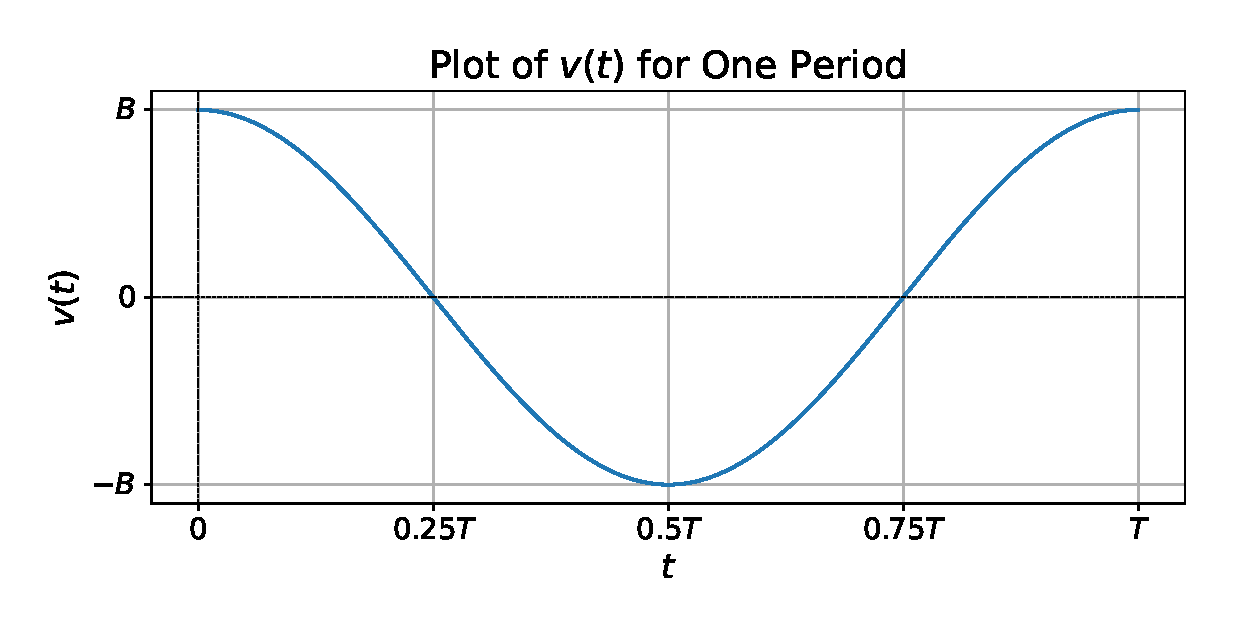
\includegraphics[width=0.9\linewidth]{figs/fig_sol_1.4b.eps}  % Replace with "plot.eps" if using EPS
  %  \caption{Plot of $v(t)$ for one period.}
 %   \label{fig:v_plot}
\end{figure}


\subsubsection*{Problem 1.5 - A damped oscillating spring}
An object of mass 0.2\,kg is hung from a spring whose spring constant is 80\,N/m. The object is subject to a resistive force given by $-bv$, where $v$ is its velocity in meters per second.
\begin{enumerate}
    \item[(a)]Set up the differential equation of motion for free oscillations of the system.
    \item[(b)]If the damped frequency is 0.995 of the undamped frequency, what is the value of the constant $b$?
    \item[(c)]What is the $Q$ of the system, and by what factor is the amplitude of the oscillation reduced after 4 complete cycles?
    \item[(d)]Which fraction of the original energy is left after 4 oscillations?
\end{enumerate}
\textbf{Solution(a)}
\\
\\Applying Newton's second law to the system:
\[F_{\text{net}}=F_{\text{spring}}+F_{\text{resistive}}\Rightarrow ma=-kx-bv\]
\[\Rightarrow\frac{d^2x}{dt^2}=-kx-b\frac{dx}{dt}\Rightarrow \frac{d^2x}{dt^2}+\frac{b}{m}\frac{dx}{dt}+\frac{k}{m}x=0\]
\[\Rightarrow \frac{d^2x}{dt^2}+\gamma\frac{dx}{dt}+\omega_0^2x=0\]
where $\gamma=b/m$ and $\omega_0^2=k/m$.
\\
\\\textbf{Solution(b)}
\\
\\Damped frequency, $\omega$, is given by the expression
\begin{equation}
    \omega^2=\omega_0^2-\frac{\gamma^2}{4}.
\end{equation}
Given that damped frequency is equal to $0.995\omega_0$ where $\omega_0$ is the undamped frequency. Substituting this value, $b/m$ for $\gamma$ and $k/m$ for $\omega_0$ into equation (4) gives
\[\left(0.995\sqrt{\frac{k}{m}}\right)^2=\frac{k}{m}-\frac{b^2}{4m^2}\Rightarrow 0.01k=\frac{b^2}{4m}\Rightarrow b=\sqrt{0.04km}=0.8\,\text{kgs}^{-1}.\]
\textbf{Solution(c)}
\\
\\Quality $Q$ is given by
\[Q=\frac{\omega_0}{\gamma}=\frac{\sqrt{k/m}}{b/m}=\frac{\sqrt{80/0.2}}{0.8/0.2}=5.\]
Factor responsible for damping is $e^{-\frac{\gamma}{2}t}$. After 4 complete cycles, a time $t=\frac{8\pi}{\omega}=1.263\,$s has passed. Thus, the amplitude after 4 complete cycles is
\[A_{4T}=A_0e^{-(\frac{0.8/0.2}{2}\times1.263)}\Rightarrow \frac{A_{4T}}{A_0}\approx0.08.\]
The amplitude has decreased to 80\% of the initial value.
\\
\\\textbf{Solution(d)}
\\
\\Energy after 4 oscillations is
\[E_{4T}=E_0e^{-\gamma t}\Rightarrow \frac{E_{4T}}{E_0}=e^{-\frac{0.8}{0.2}\times1.263}\approx0.0064.\]
Energy has decreased to 0.64\% of its initial value.

\subsubsection*{Problem 1.6 - A physical pendulum}
A uniform rod of mass $m$ is bent in a circular arc with radius $R$. It is suspended in the middle and it can freely swing about point $P$ (see Figure). The length of the arc is $\frac{2}{3}\pi R$.
\begin{figure}[h]
    \centering
    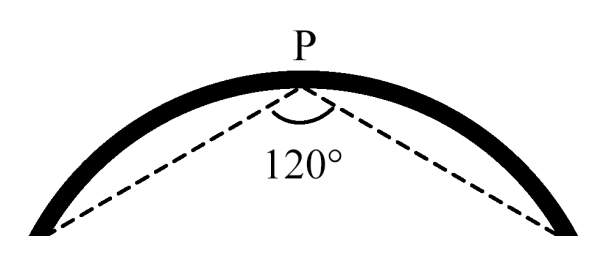
\includegraphics[width=0.4\linewidth]{figs/fig_prob_1.6.png}
  %  \caption{Caption}
 %   \label{fig:enter-label}
\end{figure}
\begin{enumerate}
    \item[(a)]What is the period of small angle oscillations about $P$?
    \item[(b)]Compare your result with the period derived (and demonstrated) in lectures for a hoop with mass $m$ and radius $R$.
\end{enumerate}
\textbf{Solution(a)}
\\
\\To solve this problem, we consider a simpler version in which the whole mass is equally divided and concentrated at both ends of this circular arc ($m/2$ at each end). Both masses ($M_1$ and $M_2$) subtend an angle $\beta$ at $P$. The moment of inertia about point $P$ of these masses would be
\[I_P=\frac{ml^2}{2}+\frac{ml^2}{2}=ml^2\]
where $l$ is the distance of each mass from $P$. If we displace this system by a small angle $theta$ in the anticlockwise direction, there will be a restoring torque on both masses due to their respective weights.
\[\boldsymbol{\Vec{\tau_{\text{net}}}}=\boldsymbol{\Vec{\tau_1}}+\boldsymbol{\Vec{\tau_2}}=M_1\boldsymbol{\Vec{l}}\times\boldsymbol{\Vec{g}}-M_2\boldsymbol{\Vec{l}}\times\boldsymbol{\Vec{g}}\]
\[=\frac{m}{2}lg\sin\left(\frac{\beta}{2}-\theta\right)-\frac{m}{2}lg\sin\left(\frac{\beta}{2}+\theta\right)\]
\[=\frac{m}{2}lg\left(\sin\frac{\beta}{2}\cos\theta-\cos\frac{\beta}{2}\sin\theta-\sin\frac{\beta}{2}\cos\theta-\cos\frac{\beta}{2}\sin\theta\right)\]
\begin{equation}
    =-mlg\cos\frac{\beta}{2}\sin\theta.
\end{equation}
From geometry, we find that $\cos\frac{\beta}{2}=\frac{l}{D}$. Since $\theta$ is small, $\sin\theta\approx\theta$ is a very good approximation. Now, the resultant torque (which is into the page) found in equation (5) becomes
\[\boldsymbol{\Vec{\tau_{\text{net}}}}=-\frac{ml^2g}{D}\theta.\]
Given that this expression is also equal to $I_P\alpha$, where $\alpha$ is the angular acceleration.
\[I_P\alpha=-\frac{ml^2g}{D}\theta\Rightarrow ml^2\ddot{\theta}=-\frac{ml^2g}{D}\theta\]
\begin{equation}
   \Rightarrow\ddot{\theta}+\frac{g}{D}\theta=0.
\end{equation}
Equation (6) shows a simple harmonic oscillation with period
\begin{equation}
    T=2\pi\sqrt{\frac{D}{g}}=2\pi\sqrt{\frac{2R}{g}}.
\end{equation}
Since the period is independent of mass $m$ and angle $\beta$, the period of actual system is same as found in equation (7). 
\\
\\\textbf{Solution(b)}
\\
\\The period found in part (a) is exactly the same as of the hoop (derived in lecture 1). 

\subsubsection*{Problem 1.7 - Damped oscillator and initial conditions}
The displacement from equilibrium, $s(t)$, of the pen of a chart recorder can be modelled as a damped harmonic oscillator satisfying the homogeneous differential equation
\[\ddot{s}(t)+\gamma\dot{s}(t)+\omega_0^2s(t)=0\]
\begin{enumerate}
    \item[(a)]Find the time evolution of the displacement if the pen is critically damped and subject to the initial conditions $s(t=0)=0$ and $\dot{s}(t=0)=v_0$. Does $s(t)$ change sign before it settles to its equilibrium position at $s=0$?
    \item[(b)]Find the response of an overdamped pen subject to the initial conditions $s(t=0)=s_0$ and $\dot{s}(t=0)=0$.
    \item[(c)]Use your favorite mathematical tool to plot your solution for $s(t)$ in (b) as a function of time. Use $\omega_0=3/7\times\pi$, $\gamma=3$ and $s_0=1$ for the plot you turn in. Let time run from 0 to 10 seconds. For your own curiosity, once you have your code written, you can vary $\gamma$ to see the effect of the damping on the response.
\end{enumerate}
\textbf{Solution(a)}
\\
\\For a critically damped system, the position of pen as a function of time is
\[s(t)=(A+Bt)e^{-\frac{\gamma}{2}t}\]
\[\dot{s}(t)=-\frac{\gamma}{2}(A+Bt)e^{-\frac{\gamma}{2}t}+Be^{-\frac{\gamma}{2}t}.\]
$s(t=0)=0$ means $A=0$ and $\dot{s}(t=0)=v_0$ leads to $B=v_0$. Thus, the time evolution of displacement in this scenario is
\[s(t)=v_0te^{-\frac{\gamma}{2}t}.\]
$s(t)$ never changes sign during the entire course of motion.
\\
\\\textbf{Solution(b)}
\\
\\The solution for an overdamped system is of the form
\[s(t)=Ae^{-\left(\gamma/2+\alpha\right)t}+Be^{-\left(\gamma/2-\alpha\right)t}\]
\[\dot{s}(t)=-\left(\gamma/2+\alpha\right)Ae^{-\left(\gamma/2+\alpha\right)t}-\left(\gamma/2-\alpha\right)Be^{-\left(\gamma/2-\alpha\right)}\]
using the initial conditions stated in the problem, we obtain
\[s(t=0)=s_0=A+B\Rightarrow B=s_0-A\]
and
\[\dot{s}(t=0)=0=-\left(\gamma/2+\alpha\right)A-\left(\gamma/2-\alpha\right)B\]
\[-\left(\gamma/2+\alpha\right)A-\left(\gamma/2-\alpha\right)(s_0-A)=0\Rightarrow A\gamma/2+A\alpha=\alpha s_0-A\alpha-\gamma s_0/2+A\gamma/2\]
\[2A\alpha=s_0\left(\alpha-\gamma/2\right)\Rightarrow A=s_0\left(\frac{\alpha-\gamma/2}{2\alpha}\right)=s_0\left(\frac{1}{2}-\frac{\gamma}{4\alpha}\right)\]
\[B=s_0-s_0\left(\frac{1}{2}-\frac{\gamma}{4\alpha}\right)=s_0\left(\frac{1}{2}+\frac{\gamma}{4\alpha}\right).\]
Finally,
\[s(t)=s_0\left(\frac{1}{2}-\frac{\gamma}{4\alpha}\right)e^{-\left(\gamma/2+\alpha\right)t}+s_0\left(\frac{1}{2}+\frac{\gamma}{4\alpha}\right)e^{-\left(\gamma/2-\alpha\right)t}\]
where
\[\alpha=\sqrt{\frac{\gamma^2}{4}-\omega_0^2}.\]
\textbf{Solution(c)}
\begin{figure}[h!]
    \centering
    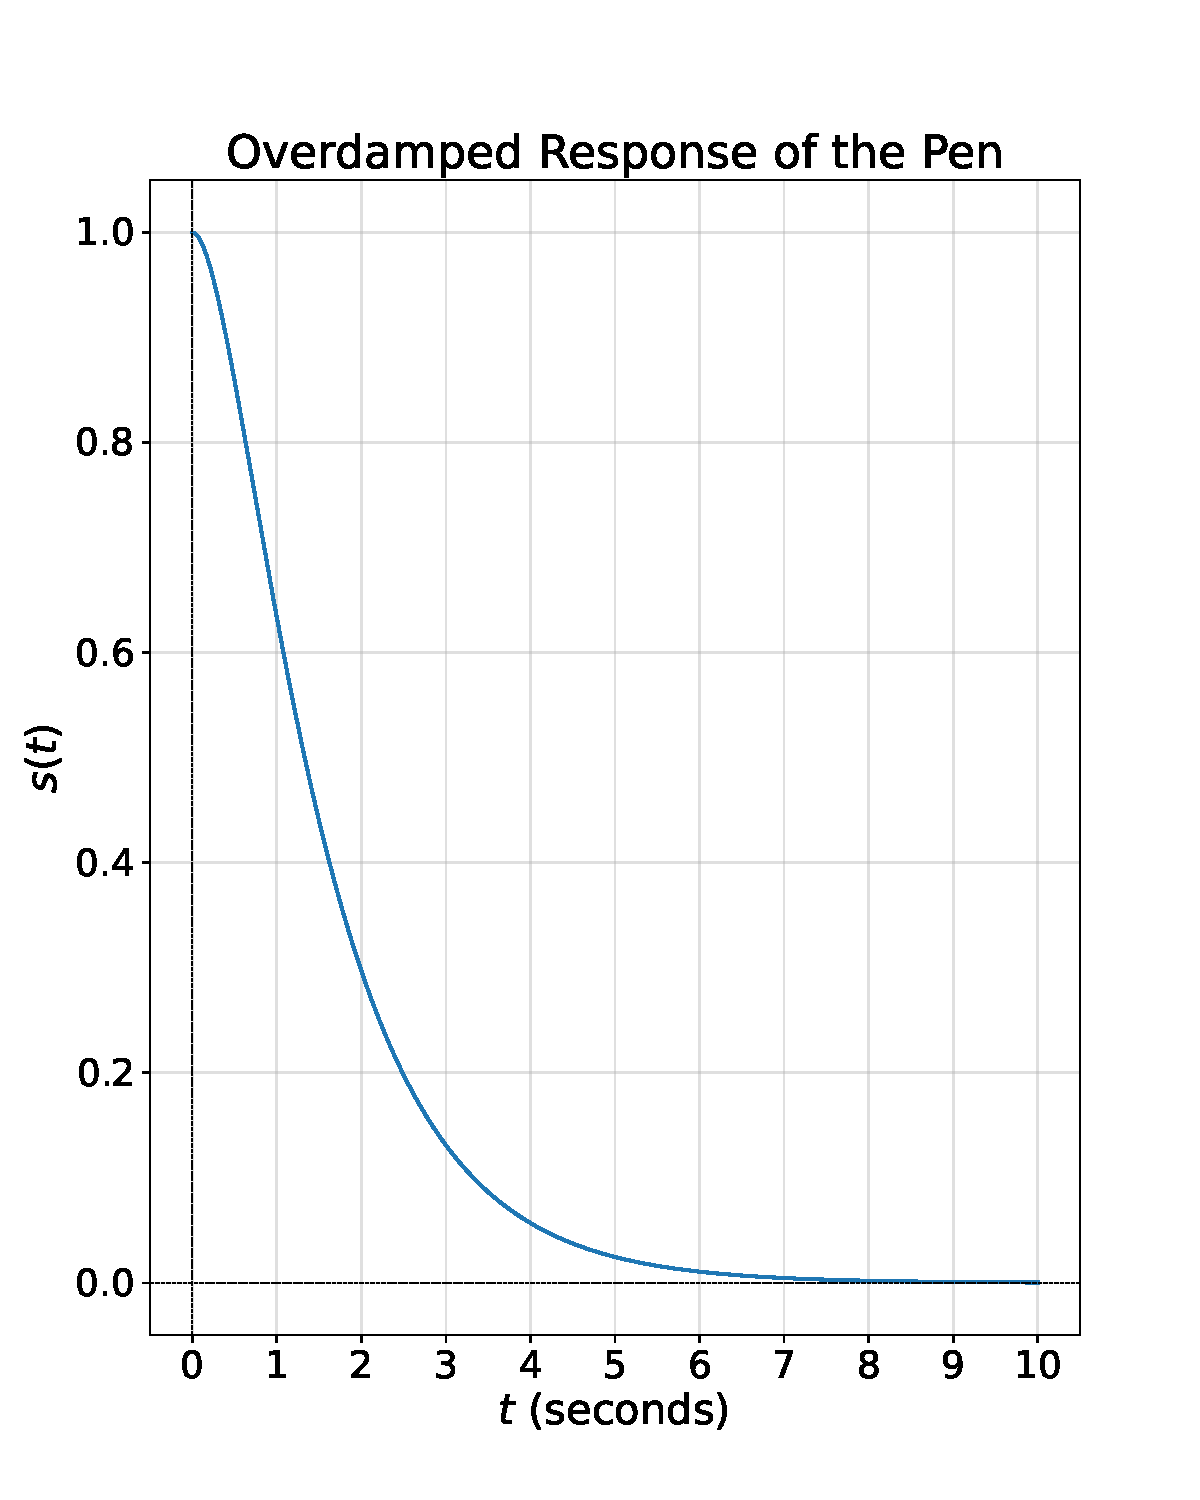
\includegraphics[width=0.8\linewidth]{figs/fig_sol_1.7c.pdf}
    %\caption{Caption}
   % \label{fig:enter-label}
\end{figure}

\end{document}